\section{Sound analysis}
In sound analysis, one can either analyze the raw sound files directly or convert them to simpler files and hope we have not lost any essential features. A big advantage with the latter, is that the dimensionality and complexity of the data set is significantly reduced, but we will also loose some information. In this section we will first introduce the Urban Sound Challenge, and then look at the sounds from a time perspective, frequency perspective and see how to extract information. Finally, we take a look at some of the samplings and see if we can classify them with the naked eye.

\subsection{The Urban Sound Challenge (USC)}
The Urban Sound Challenge is a classification contest provided by Analytics Vidhya with the purpose of introducing curious people to a real-world classification problem. After registered, one is provided with a dataset containing sounds from ten classes. For the training data set, the classes (targets) are given, but there is also a test dataset where the targets are unknown. Our task is to classify the test dataset correctly, and by uploading our results to Analytics Vidhya's webpage, they will return the accuracy score. Participants are expected to summit their answers by 31st of December 2018, and there will be a leaderboard. We are allowed to use all possible tools, including open-source libraries like TensorFlow/Keras and Scikit-Learn. For more practical information, see \cite{USC}.

The data sets consist of a total number of 8732 sound samplings (5434 training samplings and 3298 test samplings) with a constant sampling rate of 22050Hz. The length of each sampling is maximum 4 seconds, and they are distributed between ten classes, namely
\begin{multicols}{2}
	\begin{itemize}
		\setlength\itemsep{0.2em}
		\item air conditioner
		\item car horn
		\item children playing
		\item dog bark
		\item drilling
	\end{itemize}
	
	\columnbreak
	
	\begin{itemize}
		\setlength\itemsep{0.2em}
		\item engine idling
		\item gun shot
		\item jackhammer
		\item siren
		\item street music.
	\end{itemize}
\end{multicols}

The error is evaluated with the accuracy score, which is just how much of the data set that is classified correctly:
\begin{empheq}[box={\mybluebox[5pt]}]{equation}
\text{Accuracy}=\frac{\sum_{i=1}^NI(y_i=t_i)}{N}.
\end{empheq}

\subsection{Time domain}
Sounds are longitudinal waves which actually are different pressures in the air. They are usually represented as a function in the time domain, which means how the pressure vary per time. This function is obviously continuous, but since computers represent functions as arrays, we cannot save all the information. 

\begin{figure} [H]
	\centering
	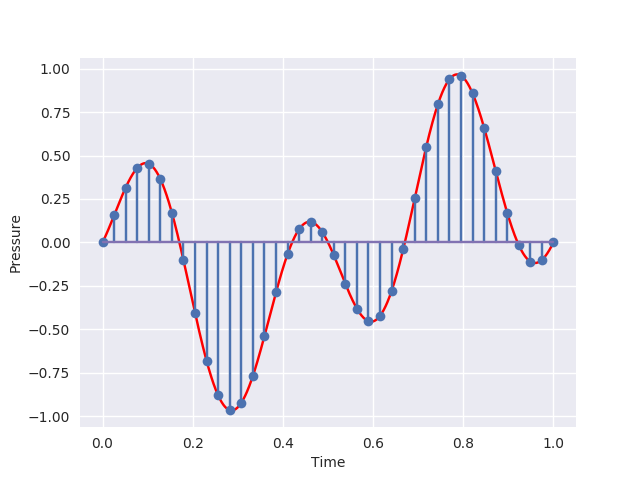
\includegraphics[scale=0.9]{../plots/sampling_rate.png}
	\caption{When sampling sound, we need to choose a high enough sampling. Here, the red line is the true sound and the blue dots are sampling points. The sampling rate here is 40 Hz, which is quite low and just for illustration.}
	\label{fig:sr}
\end{figure} 

How much information we loose depends on the sampling rate, which is the number of sampling points per second (see figure \eqref{fig:sr}). A rule of thumb is that one should have twice as high sampling rate as the highest sound frequency to keep the most important information. For instance, a human ear can perceive frequencies in the range 20-20000Hz, so around a sampling rate around 40kHz should be sufficient to keep all the information. Ordinary CD's use a sampling rate of 44.1kHz, but for speech recognition, 16kHz is enough to cover the frequency range of human speech. \cite{Medium}

\subsection{Frequency domain}
Sometimes, a frequency domain gives a better picture than the time domain. On one hand, one looses the time dependency, but on the other one gets information about which frequencies that are found in the wave. To go from the time domain to the frequency domain, one needs to use Fourier transformations, defined by 
\begin{empheq}[box={\mybluebox[5pt]}]{equation}
\hat{f}(x)=\int_{-\infty}^{\infty}f(t)\exp(-2\pi ixt)dx
\end{empheq}
where $f(t)$ is the time function and $\hat{f}(x)$ is the frequency function. Fortunately we do not need to solve this analytically, Fast Fourier Transformations (FFT) does the job numerically in no time. In figure \eqref{fig:freq}, FFT is used on a time picture to obtain the corresponding frequency picture.  

\begin{figure} [H]
	\centering
	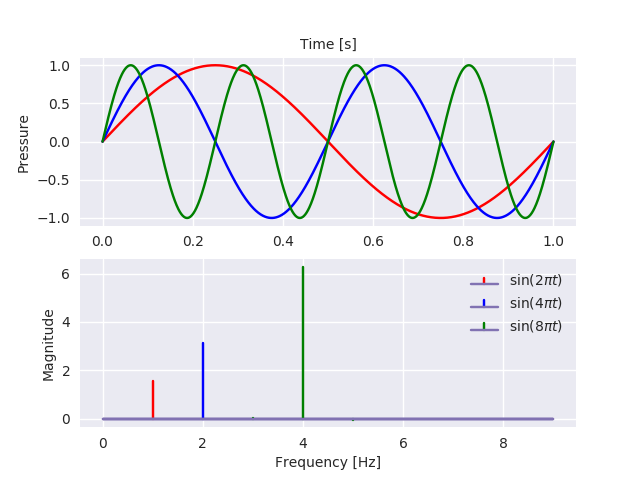
\includegraphics[scale=0.9]{../plots/frequency_domain.png}
	\caption{Time picture of three harmonic functions; $\sin(2\pi t)$, $\sin(4\pi t)$ and $\sin(8\pi t)$ (upper part) and the corresponding frequency pictures (lower part).}
	\label{fig:freq}
\end{figure} 
\newpage

\subsection{Extract features}
There are many ways we can extract features from sound, but the most interesting are those that are based on how humans extract information. First the spectrogram method will be described briefly, and we thereafter turn to the mel frequency ceptral coefficients method. 

\subsubsection*{Spectrograms}
As we have seen above, we are missing the frequency information in the time domain, and time information in the frequency domain. Is it possible to get the best of both worlds? This is what we try when creating a spectrogram, which is a time-frequency representation. 

The procedure goes like this: we divide the spectrum into $N$ frames and Fourier transform each frame. Thereafter we collect all the frequency domains in a $NxM$-matrix, where $M$ is the length of each frequency domain. We are then left with an image which hopefully hold the important information, and since Hidden Markov Models are known to implicity model spectrograms for speech recognition, we have a reason to believe it will work. \cite{spectrograms}

\subsubsection*{Mel Frequency Cepstral Coefficients (MFCCs)}
MFCCs are features widely used in automatic speech and speaker recognition. \cite{mfcc} They are inspired by how the human ear extracts features, and has been the main feature extraction tool for sound recognition since it was introduced in the 1980's. 

It actually takes advantage of the spectrogram, and use it to reveal the most dominant frequencies. Thereafter, we sum the energy in each frame and take the logarithm, which is the way an ear works. Those energies are then what we call the Mel Frequency Ceptral Coefficients. Unlike the spectrogram, we are now left with a single array of information from the spectrum. 

\subsection{Examples from USC}
We will end this section with a few examples of what a sound file may look like. In figure \eqref{fig:comparison}, we compare one of the dog bark sounds with one of the jackhammer sounds. On the top, we have the time domain, in the middle the spectrogram is presented and on the bottom we have plotted the MFCCs. As we can see, they are quite different, and distinguish between those two should not be too hard. The spectrograms also really makes sense, but it is hard for a human eye to extract information from the MFCCs. 

\begin{figure} [H]%
	\centering
	\subfloat[Dog bark]{{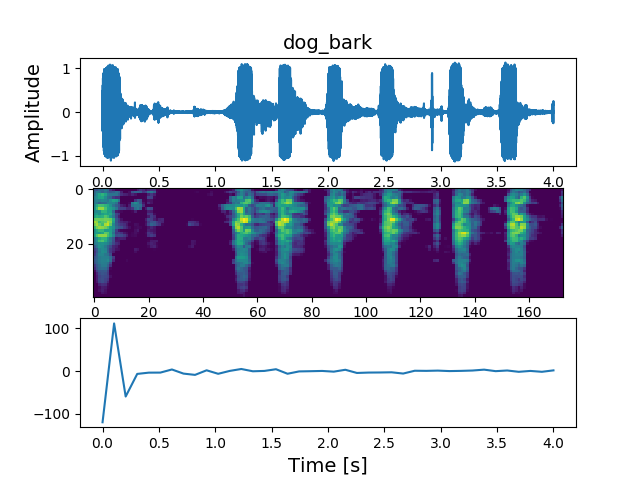
\includegraphics[width=7.8cm]{../plots/dog_bark_comp.png}}}
	\subfloat[Jackhammer]{{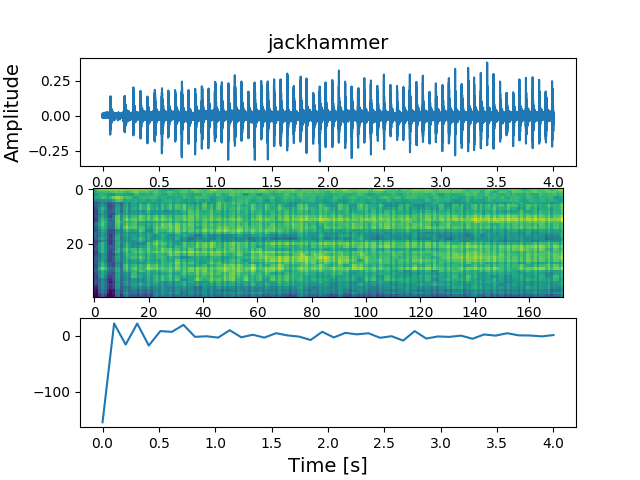
\includegraphics[width=7.8cm]{../plots/jackhammer_comp.png}}}
	
	\caption{Time domains (top), spectrograms (middle) and MFCCs (bottom) for two random sound files, more specifically dog bark on the left and jackhammer on the right.}%
	\label{fig:comparison}
\end{figure}
However, sometimes two time domains in the same category look totally different, for example if one compares the jackhammer in \eqref{fig:comparison2} with the one in \eqref{fig:comparison}. Will it be possible for our program to understand that they are in the same category? Also sometimes two time domain from different categories look similar, as we can see in \eqref{fig:comparison2}. Can we really distinguish between them?

\begin{figure} [H]%
	\centering
	\subfloat[Jackhammer]{{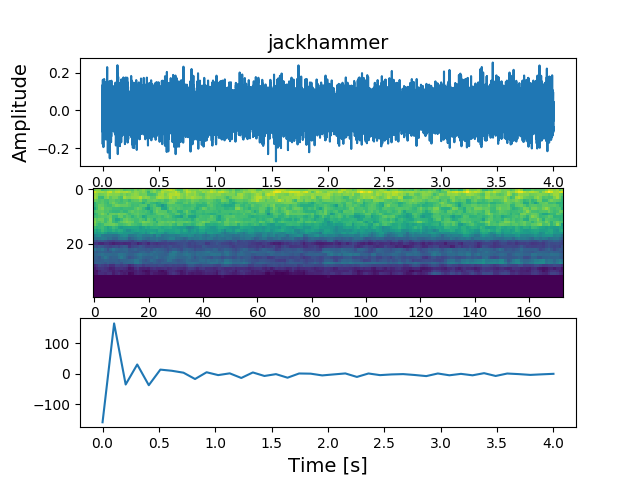
\includegraphics[width=7.8cm]{../plots/jackhammer_comp2.png}}}
	\subfloat[Drilling]{{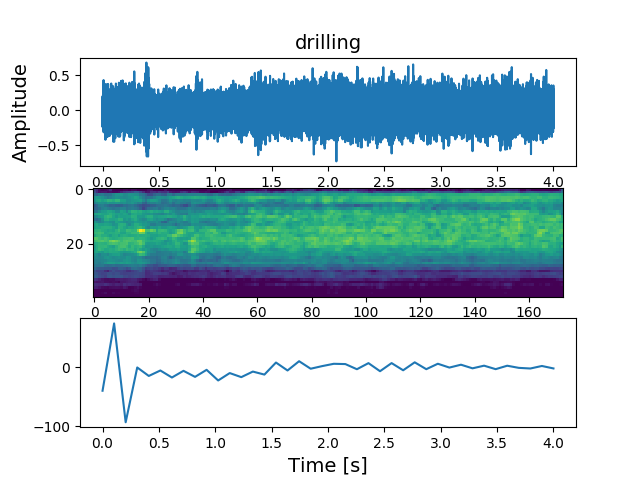
\includegraphics[width=7.8cm]{../plots/drilling_comp2.png}}}
	
	\caption{Time domains (top), spectrograms (middle) and MFCCs (bottom) for two random sound files, more specifically jackhammer on the left and drilling on the right.}%
	\label{fig:comparison2}
\end{figure}